\documentclass[11pt]{article}
\usepackage[final]{acl}
\usepackage{times}
\usepackage{latexsym}
\usepackage[T1]{fontenc}
\usepackage[utf8]{inputenc}
\usepackage{microtype}
%\usepackage{inconsolata}  % not installed locally
\usepackage{graphicx}
\usepackage{booktabs}
\usepackage{amsmath}
\usepackage{xspace}

\newcommand{\ours}{\textsc{LADL}\xspace}
\newcommand{\st}[1]{\texttt{#1}}

\title{Beyond Remembering: Maintaining Active Constraints and Pending\\ Commitments Across Context Compaction}

\author{Sheng Lu \quad Qixiang Fan \quad Ziyan Fan \quad Xiuping Zhu \\
  Georgia Institute of Technology \\
  \texttt{ECE 6256 / CS 6604, Fall 2026}}

\begin{document}
\maketitle

\begin{abstract}
Long-running conversational agents must track more than facts: a prohibition may be lifted, an approval condition may become satisfied, and a promised action may already have been carried out. Context compaction can blur these distinctions and induce wrong tool calls. We study whether explicit lifecycle tracking improves action correctness under repeated compaction. Our Lifecycle-Aware Dialogue Ledger (\ours) records prohibitions and commitments as typed items whose status is updated by a deterministic, evidence-grounded reducer. We build a controlled benchmark of 192 dialogues (48 gold event timelines, 24--42 turns, 1--5 compaction rounds, 872 decision probes) with programmatically verified state timelines, and compare full history, ordinary compaction, constraint pinning, a chronological event ledger and a typed ledger with LLM-written transitions under a matched 384-token memory budget. With Qwen2.5-7B, \ours raises action accuracy from 60.1\% (ordinary compaction) and 64.2\% (pinning) to 76.4\% and halves constraint violations. With Llama-3.1-8B the gain does not materialize (71.1\% vs.\ 73.5\%): a gold-event ledger reaches 81.5\%, and our error attribution traces the gap to extraction of a single fine-grained field that the deterministic rules then amplify. Across conditions, mutable state that is not lost tends to become \emph{stale} rather than missing, even with full history in context.
\end{abstract}

\section{Introduction}

Conversational memory is usually evaluated by asking what an assistant recalls. The operational question for a tool-using agent is often different: \emph{what is it still authorized or obliged to do?} Consider ``Do not send the report until I approve the final version.'' Approving the outline does not satisfy the guard; an explicit final approval activates the commitment; a successful tool receipt discharges it, after which a reminder must not trigger a duplicate send. After the conversation is compacted into a summary, an agent can forget the guard, treat an obsolete restriction as active, or repeat a completed action---even when the relevant text has nominally been retained.

Prior work shows that compaction silently drops side constraints and safety rules \citep{wang2026lost,zerhoudi2026cliff,chen2026governance}, and that pinning protected text prevents some resulting violations \citep{chen2026governance}. These studies treat constraints as static. We focus on state that changes \emph{after} it is stated, and ask:

\textbf{RQ1.} Static constraints decay under repeated compaction; does mutable state (revoked, triggered, discharged items) degrade differently---e.g.\ by becoming \emph{stale} rather than \emph{missing}?\\
\textbf{RQ2.} Under an equal memory budget, does explicit lifecycle tracking improve downstream action correctness over pinning and chronological memory?\\
\textbf{RQ3.} Which errors arise from incorrect stored state versus incorrect decisions given correct state?

Our contributions are: (i) a controlled benchmark with gold event timelines, programmatic state labels and permissible actions at every probe (\S\ref{sec:data}); (ii) \ours, a lightweight ledger with a deterministic transition reducer (\S\ref{sec:method}); (iii) a matched-budget comparison against five memory conditions on two open 7--8B models, with timeline-clustered confidence intervals, ablations of the transition logic, a gold-state intervention, and error attribution (\S\ref{sec:results}). We find a large gain for one model and none for the other, and we use the attribution analysis to explain why.

\section{Related Work}

LoCoMo and LongMemEval characterize long-term conversational recall, including temporal updates \citep{maharana2024locomo,wu2025longmemeval}; MemGPT manages bounded context by paging memory \citep{packer2023memgpt}. Closest to us, \citet{wang2026lost} show that current compactors often omit side constraints, \citet{zerhoudi2026cliff} find that safety-rule recall decays over successive compaction rounds, and \citet{chen2026governance} show that dropped governance constraints cause prohibited tool calls that Constraint Pinning prevents. LedgerAgent maintains structured task state and gates tool calls against it \citep{uddin2026ledgeragent} but does not study compaction or state that evolves. MEME evaluates evolving multi-entity memory \citep{jung2026meme}, and Mem2ActBench evaluates memory-grounded tool use \citep{shen2026mem2act}. Our gap is their intersection: revoked prohibitions and triggered or discharged commitments under repeated compaction, scored at tool-decision checkpoints. We do not claim that structured state or pinning is new; we test whether lifecycle-aware transitions matter beyond them.

\section{Benchmark}
\label{sec:data}

\paragraph{Event model.} Each dialogue concerns a workplace assistant with eight mock tools (email, file sharing, chat posts, bookings, orders, payments, publishing, deletion). Items are \emph{prohibitions} or \emph{commitments}. Seven event types change state: \st{prohibit} (create or reinstate), \st{revoke}, \st{ambiguous} (the user hedges and asks to be consulted), \st{commit} (with an optional guard), \st{approve} (with the approved object), \st{cancel}, and \st{tool\_result} (success/failure receipts).

\paragraph{Timeline families.} We hand-wrote 13 families covering the three proposal categories: \emph{revocation} (revoke; revoke then reinstate; hedge then revoke; revoke one of two prohibitions), \emph{completion followed by repeat requests} (success; failure; failure then retry; triggered-then-success; triggered-then-failure), and \emph{conditional triggering} (partial then final approval; only partial approvals; hedged approval; cancelled then approved ``for the records''). Each of 48 timelines interleaves a primary family, a secondary family from another category and a \emph{static} control prohibition that never changes, with one distinct tool per item.

\paragraph{Rendering and labels.} Events are rendered with utterance templates (even-indexed templates for dev, odd-indexed held-out templates for test) and interleaved with coherent filler, 20\% of which mentions an item's document without changing state. Each timeline yields four dialogues with 1, 2, 3 or 5 compaction points spread over the dialogue; two of the four variants are paraphrased by Llama-3.1-8B. A paraphrase is accepted only if it keeps entity words and polarity cues \emph{and} an equivalence judge (Qwen2.5-7B) confirms the meaning (32\% acceptance); a manual audit of 40 accepted paraphrases found 38 meaning-preserving, one label error and one borderline case. Decision probes arrive from teammates, a workflow engine or reminders---never from the user, so a request cannot itself be read as a revocation---and the agent's answer is not fed back, keeping labels deterministic. The gold reducer (\S\ref{sec:method}) produces the item state at each probe, and fixed rules map it to the permissible decision: \st{decline} (prohibition active, cancelled, or completed), \st{wait} (guard unmet), \st{clarify} (latest user statement hedged), or \st{act} (unrestricted, revoked, ready, or retry after failure). The final set has 192 dialogues (mean 32.7 turns) and 872 probes; the dev split (12 timelines, 208 probes) was used only for prompt development, and all results are on the 36 test timelines (144 dialogues, 664 probes).

\section{Method: Lifecycle-Aware Dialogue Ledger}
\label{sec:method}

\paragraph{Extraction.} For every user and tool turn, an LLM extractor sees the tool list, the current item registry (IDs, actions and guards, but not statuses), the two previous turns and the new turn, and emits zero or more typed events with JSON-schema-constrained decoding. Approvals carry \st{explicit} and \st{matches\_guard} flags. The registry assigns stable IDs and resolves dangling references by tool and target similarity.

\paragraph{Reducer.} A deterministic reducer maintains each item's status: \st{active}/\st{revoked} for prohibitions and \st{waiting}/\st{ready}/\st{completed}/\st{cancelled} for commitments, plus an \emph{unclear} flag and a failed-attempt counter. Only an explicit approval that satisfies the stored guard moves a commitment to \st{ready}; only a verified tool success moves it to \st{completed}; a failure leaves it pending; approvals of cancelled items are ignored; ambiguous updates set \emph{unclear} rather than granting permission. Every transition, and every rejected one (e.g.\ ``approval of the outline does not satisfy guard''), is logged with its evidence turn.

\paragraph{Compaction and policy.} At each compaction point the dialogue so far is replaced by a recursive task-focused summary, while a rendered current-state ledger persists alongside it. Summary plus ledger share one budget $B$ (default 384 tokens; the persistent block may use at most $0.6B$). At a probe, the action policy sees memory, the turns since the last compaction and the request, writes the user's relevant instructions and their current status, and outputs \st{act}, \st{wait}, \st{clarify} or \st{decline}. A separate \emph{state query} asks the same model for the item's status (8 labels incl.\ \emph{unknown}), which lets us measure recall in conditions without explicit state.

\section{Experimental Setup}

\paragraph{Conditions.} (1) \textbf{Full} history without compaction (diagnostic reference); (2) \textbf{ordinary} task-focused compaction; (3) \textbf{constraint pinning}: a pinned-rules text that the LLM rewrites after every user/tool turn, so it can also record lifted or completed rules; (4) a \textbf{chronological event ledger} of the same extracted events without states (oldest entries dropped at the budget); (5) the same \textbf{typed ledger with LLM-written transitions}; (6) \textbf{\ours}. Conditions 2--6 share the event stream, the budget, the summarizer, the policy prompt and the model. We also run \ours on \textbf{gold events} (the gold-state intervention, which also upper-bounds extraction), and ablate guard logic (any approval triggers) and receipt evidence (any attempt completes).

\paragraph{Models and inference.} Qwen2.5-7B-Instruct and Llama-3.1-8B-Instruct serve as summarizer, extractor and policy for their own runs, using vLLM \citep{kwon2023vllm} at temperature 0 with all calls cached for exact reproducibility. Prompts were developed on the dev split and frozen before the test runs. Each main run (nine conditions, 664 probes, about 20.7k LLM calls and 14--15M prompt tokens) took 19 min (Qwen) and 28 min (Llama) on one NVIDIA RTX 6000 Ada (48GB). We ran on a local two-GPU workstation rather than PACE-ICE because it was available and needed no queueing; a PACE job script is included.

\paragraph{Metrics and statistics.} The primary metric is action accuracy. Error rates are computed on the probes where they can occur: \emph{violation} (act when prohibited or cancelled), \emph{over-restriction} (wait/decline when act is permitted), \emph{premature} (act while the guard is unmet) and \emph{duplicate} (act after verified completion). We report 95\% percentile bootstrap CIs (2{,}000 resamples) resampling timelines, so all dialogues and probes of a timeline move together, and paired differences on identical probes.

\section{Results}
\label{sec:results}

\begin{table}[t]
\centering\small\setlength{\tabcolsep}{3pt}
\resizebox{\columnwidth}{!}{\begin{tabular}{lrrrrrr}
\toprule
 & \multicolumn{3}{c}{Qwen2.5-7B} & \multicolumn{3}{c}{Llama-3.1-8B} \\
\cmidrule(lr){2-4}\cmidrule(lr){5-7}
Condition & Acc. & 95\% CI & State & Acc. & 95\% CI & State \\
\midrule
Full history (no compaction) & 60.4 & [55.2, 64.9] & 73.5 & 81.6 & [77.9, 84.8] & 76.1 \\
Ordinary compaction & 60.1 & [56.3, 63.7] & 64.5 & 73.5 & [70.2, 76.7] & 64.6 \\
Constraint pinning & 64.2 & [59.5, 68.5] & 67.9 & 66.4 & [62.9, 70.2] & 63.3 \\
Chronological event ledger & 69.9 & [66.4, 73.3] & 73.9 & \textbf{77.0} & [72.4, 81.2] & 67.5 \\
Typed ledger, LLM transitions & 69.1 & [64.6, 73.4] & 72.7 & 69.4 & [65.0, 73.9] & 70.0 \\
Lifecycle ledger (\textit{ours}) & \textbf{76.4} & [72.7, 80.2] & 87.8 & 71.1 & [66.1, 76.0] & 76.7 \\
\midrule
Lifecycle ledger, gold events & 83.1 & [80.0, 85.8] & 91.4 & 81.5 & [78.2, 84.3] & 83.4 \\
Ours - guard logic & 74.5 & [70.7, 78.1] & 84.5 & 77.6 & [73.7, 81.5] & 77.3 \\
Ours - receipt evidence & 74.7 & [70.8, 78.7] & 83.4 & 68.8 & [63.1, 74.4] & 72.4 \\
Ours, strict hedging (post-hoc) & 76.1 & [72.4, 79.4] & 87.8 & 76.8 & [72.5, 81.1] & 76.7 \\
\bottomrule
\end{tabular}
}
\caption{Action accuracy (\%) with timeline-clustered 95\% CIs, and state-recall accuracy (State, \%) on 664 test probes at $B{=}384$. Bold: best compacted condition per model. Rows below the rule are diagnostics and ablations.}
\label{tab:main}
\end{table}

\begin{table}[t]
\centering\small\setlength{\tabcolsep}{3pt}
\resizebox{\columnwidth}{!}{% Generated by python -m src.eval.paper_assets; do not edit.
\begin{tabular}{lllrrc}
\toprule
Family & Model & Comparison & Difference & Holm $p$ & Confirmed \\
\midrule
Primary & Qwen2.5-7B & LADL v1 $-$ Compaction + hints & +15.9 {\scriptsize [+12.3, +19.9]} & 0.008 & yes \\
Primary & Qwen2.5-7B & LADL v1 $-$ Pinning + hints & +16.0 {\scriptsize [+12.7, +19.4]} & 0.008 & yes \\
Primary & Qwen2.5-7B & LADL v1 $-$ Chronological + hints, v1 & +7.8 {\scriptsize [+4.4, +11.2]} & 0.008 & yes \\
Primary & Qwen2.5-7B & LADL v1 $-$ LLM-written transitions, v1 & +10.0 {\scriptsize [+5.9, +14.3]} & 0.008 & yes \\
Primary & Llama-3.1-8B & LADL v1 $-$ Compaction + hints & +12.8 {\scriptsize [+9.1, +16.3]} & 0.008 & yes \\
Primary & Llama-3.1-8B & LADL v1 $-$ Pinning + hints & +6.1 {\scriptsize [+2.8, +9.3]} & 0.008 & yes \\
Primary & Llama-3.1-8B & LADL v1 $-$ Chronological + hints, v1 & +3.6 {\scriptsize [+0.0, +7.2]} & 0.106 & no \\
Primary & Llama-3.1-8B & LADL v1 $-$ LLM-written transitions, v1 & +0.0 {\scriptsize [-2.2, +2.1]} & 1.000 & no \\
Secondary & Qwen2.5-7B & LADL v1 $-$ Ordinary compaction & +18.2 {\scriptsize [+14.7, +21.9]} & 0.012 & yes \\
Secondary & Qwen2.5-7B & LADL v1 $-$ Constraint pinning & +12.6 {\scriptsize [+8.8, +16.3]} & 0.012 & yes \\
Secondary & Qwen2.5-7B & LADL v1 $-$ Chronological ledger, v1 & +7.8 {\scriptsize [+4.5, +11.0]} & 0.012 & yes \\
Secondary & Qwen2.5-7B & LADL v1 $-$ LADL v1 without hints & +4.1 {\scriptsize [+1.2, +7.2]} & 0.077 & no \\
Secondary & Qwen2.5-7B & LADL v2 $-$ LADL, extraction v1 & -0.3 {\scriptsize [-2.2, +1.4]} & 1.000 & no \\
Secondary & Qwen2.5-7B & Strict hedging $-$ LADL, extraction v1 & +0.0 {\scriptsize [+0.0, +0.0]} & 1.000 & no \\
Secondary & Llama-3.1-8B & LADL v1 $-$ Ordinary compaction & +2.5 {\scriptsize [-1.2, +6.0]} & 0.716 & no \\
Secondary & Llama-3.1-8B & LADL v1 $-$ Constraint pinning & +3.8 {\scriptsize [+0.2, +7.4]} & 0.216 & no \\
Secondary & Llama-3.1-8B & LADL v1 $-$ Chronological ledger, v1 & -2.3 {\scriptsize [-6.6, +1.5]} & 0.825 & no \\
Secondary & Llama-3.1-8B & LADL v1 $-$ LADL v1 without hints & -2.9 {\scriptsize [-6.4, +0.4]} & 0.435 & no \\
Secondary & Llama-3.1-8B & LADL v2 $-$ LADL, extraction v1 & +6.1 {\scriptsize [+3.7, +8.8]} & 0.012 & yes \\
Secondary & Llama-3.1-8B & Strict hedging $-$ LADL, extraction v1 & +4.8 {\scriptsize [+2.6, +7.3]} & 0.012 & yes \\
Primary (Mistral) & Mistral-7B & LADL v1 $-$ Compaction + hints & -1.9 {\scriptsize [-5.4, +1.7]} & 0.646 & no \\
Primary (Mistral) & Mistral-7B & LADL v1 $-$ Pinning + hints & -1.0 {\scriptsize [-4.7, +2.5]} & 0.646 & no \\
Primary (Mistral) & Mistral-7B & LADL v1 $-$ Chronological + hints, v1 & +8.3 {\scriptsize [+5.3, +11.6]} & 0.004 & yes \\
Primary (Mistral) & Mistral-7B & LADL v1 $-$ LLM-written transitions, v1 & +11.9 {\scriptsize [+8.8, +15.1]} & 0.004 & yes \\
v2 family (Mistral) & Mistral-7B & LADL v2 $-$ Ordinary compaction & -5.0 {\scriptsize [-9.9, -0.4]} & 0.062 & no \\
v2 family (Mistral) & Mistral-7B & LADL v2 $-$ Compaction + hints & -6.6 {\scriptsize [-10.5, -2.6]} & 0.007 & no \\
v2 family (Mistral) & Mistral-7B & LADL v2 $-$ Constraint pinning & -6.7 {\scriptsize [-11.3, -2.2]} & 0.028 & no \\
v2 family (Mistral) & Mistral-7B & LADL v2 $-$ Pinning + hints & -5.7 {\scriptsize [-9.9, -1.8]} & 0.015 & no \\
v2 family (Mistral) & Mistral-7B & LADL v2 $-$ Chronological ledger & +4.4 {\scriptsize [+0.5, +7.8]} & 0.060 & no \\
v2 family (Mistral) & Mistral-7B & LADL v2 $-$ Chronological + hints & +3.2 {\scriptsize [-0.2, +6.4]} & 0.074 & no \\
v2 family (Mistral) & Mistral-7B & LADL v2 $-$ LLM-written transitions & +10.2 {\scriptsize [+6.7, +13.7]} & 0.007 & yes \\
Secondary (Mistral) & Mistral-7B & LADL v1 $-$ Ordinary compaction & -0.3 {\scriptsize [-4.8, +4.2]} & 1.000 & no \\
Secondary (Mistral) & Mistral-7B & LADL v1 $-$ Constraint pinning & -2.0 {\scriptsize [-6.0, +2.3]} & 1.000 & no \\
Secondary (Mistral) & Mistral-7B & LADL v1 $-$ Chronological ledger, v1 & +8.3 {\scriptsize [+4.7, +11.9]} & 0.006 & yes \\
Secondary (Mistral) & Mistral-7B & LADL v1 $-$ LADL v1 without hints & -3.6 {\scriptsize [-6.8, -0.3]} & 0.140 & no \\
Secondary (Mistral) & Mistral-7B & LADL v2 $-$ LADL, extraction v1 & -4.7 {\scriptsize [-7.3, -2.1]} & 0.015 & no \\
Secondary (Mistral) & Mistral-7B & Strict hedging $-$ LADL, extraction v1 & +0.0 {\scriptsize [+0.0, +0.0]} & 1.000 & no \\
\bottomrule
\end{tabular}
}
\caption{Paired accuracy difference, \ours minus baseline, in percentage points with 95\% CI and two-sided bootstrap $p$.}
\label{tab:paired}
\end{table}

\paragraph{RQ2: lifecycle tracking under a matched budget.} Table~\ref{tab:main} and Table~\ref{tab:paired} give the main comparison. With \textbf{Qwen2.5-7B}, \ours is the best compacted condition by a wide margin: 76.4\% versus 60.1\% for ordinary compaction (+16.3 pp), 64.2\% for pinning (+12.2), 69.9\% for the chronological ledger (+6.5) and 69.1\% for LLM-written transitions (+7.2), all $p\le0.002$. It even exceeds full history (60.4\%), because this policy is markedly over-restrictive when reading long raw contexts (30\% over-restriction; Table~\ref{tab:errors}). Its violation rate falls from 12.5\% (ordinary) to 4.7\%, and its state recall from the same context rises from 64.5\% to 87.8\%.

With \textbf{Llama-3.1-8B} the picture is different. Full history (81.6\%) is strong, and among compacted conditions the chronological ledger is best (77.0\%); \ours (71.1\%) does not beat ordinary compaction (73.5\%, $p{=}0.35$) and only marginally beats pinning ($p{=}0.09$). Two observations locate the problem. First, with gold events the same ledger and policy reach 81.5\%, matching full history, so the representation itself is adequate. Second, \ours is worst on exactly the conditional category, where 59 of its 128 guard-unmet probes are answered \st{clarify}, 44 of them because the ledger marks the item \emph{unclear}. Llama's extractor frequently marks partial approvals (``I approve the salary section; still reviewing the rest'') as \st{explicit=false}, and our rule turns a non-explicit approval into an \emph{unclear} flag, which the policy correctly obeys. The deterministic reducer thus faithfully amplifies an extraction error in one fine-grained field. A post-hoc variant that takes clarification flags only from explicit \st{ambiguous} events (designed after inspecting these errors, checked on dev, and therefore exploratory) recovers Llama to 76.8\% (+5.7 pp over \ours, $p{<}0.001$) and leaves Qwen unchanged (76.1\%).

\begin{table}[t]
\centering\small\setlength{\tabcolsep}{2.5pt}
\resizebox{\columnwidth}{!}{\begin{tabular}{lrrrrrrrr}
\toprule
 & \multicolumn{4}{c}{Qwen2.5-7B} & \multicolumn{4}{c}{Llama-3.1-8B} \\
\cmidrule(lr){2-5}\cmidrule(lr){6-9}
Condition & Viol. & Over. & Prem. & Dup. & Viol. & Over. & Prem. & Dup. \\
\midrule
Full history (no compaction) & 3.9 & 30.2 & 0.8 & 4.4 & 4.7 & 8.3 & 10.9 & 36.8 \\
Ordinary compaction & 12.5 & 28.6 & 8.6 & 17.6 & 7.3 & 4.7 & 11.7 & 19.1 \\
Constraint pinning & 7.3 & 35.9 & 2.3 & 17.6 & 10.3 & 12.0 & 9.4 & 23.5 \\
Chronological event ledger & 11.2 & 18.8 & 3.9 & 10.3 & 10.8 & 5.2 & 10.2 & 33.8 \\
Typed ledger, LLM transitions & 7.3 & 35.4 & 11.7 & 14.7 & 9.1 & 14.6 & 8.6 & 16.2 \\
Lifecycle ledger  & 4.7 & 19.3 & 4.7 & 14.7 & 8.6 & 7.3 & 7.8 & 8.8 \\
Lifecycle ledger, gold events & 2.2 & 19.8 & 0.8 & 7.4 & 6.0 & 4.7 & 9.4 & 14.7 \\
\bottomrule
\end{tabular}
}
\caption{Error rates (\%) on the probes where each error can occur: violation, over-restriction, premature action, duplicate execution.}
\label{tab:errors}
\end{table}

\paragraph{Error profiles.} Table~\ref{tab:errors} shows that the conditions fail differently. Duplicate execution is common even with full history for Llama (36.8\%) and for the chronological ledger (33.8\%), which lists the success receipt but leaves its implication to the policy; \ours cuts Llama's duplicates to 8.8\%. Pinning gives Qwen few premature actions (2.3\%) but the highest over-restriction (35.9\%); its accuracy is lowest on lifted prohibitions (62.0\%) and on retries after failure (31.2\%), i.e.\ the rewritten rule text keeps restricting actions whose status has moved on. LLM-written transitions produce the most premature actions for Qwen (11.7\%), i.e.\ the LLM promotes commitments to ready on partial approvals---the error the guard rule exists to prevent.

\begin{figure*}[t]
\centering
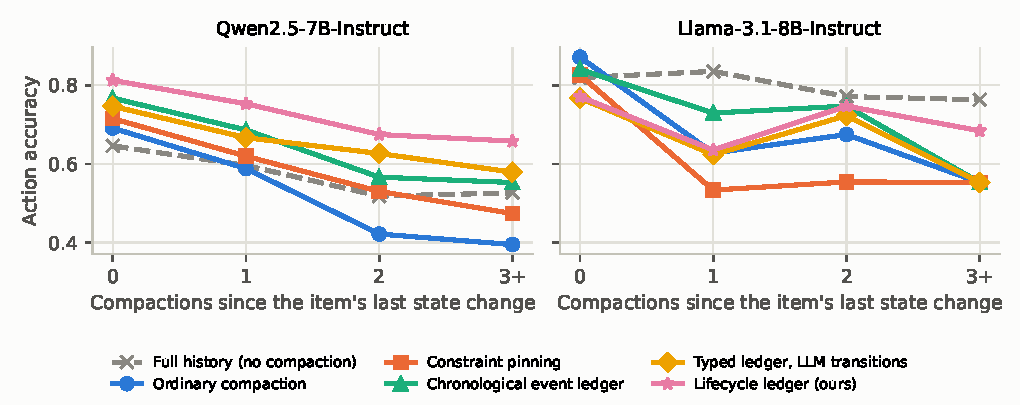
\includegraphics[width=0.85\textwidth]{figures/fig_decay.pdf}
\caption{Action accuracy as a function of the number of compactions between the probed item's last state change and the probe (test split, $B{=}384$).}
\label{fig:decay}
\end{figure*}

\paragraph{Decay with repeated compaction.} Figure~\ref{fig:decay} plots accuracy against the number of compactions between the item's last transition and the probe. Ordinary compaction decays steeply for both models (Qwen 69\%$\to$40\%, Llama 87\%$\to$55\% from 0 to $\ge$3 compactions), as does pinning. \ours decays less (Qwen 81\%$\to$66\%, Llama 77\%$\to$68\%), so its relative advantage is largest exactly where compaction has acted repeatedly. Its residual decline comes from the summary and policy rather than the ledger, which was truncated at only 0.1\% of probes (versus 13.8\% for the chronological log, whose oldest events are dropped first).

\paragraph{RQ1: stale versus missing.} The state query lets us classify recall errors as \emph{missing} (``unknown''), \emph{stale} (a status the item really had earlier) or \emph{other}. Table~\ref{tab:rq1} restricts to probes with at least one compaction since the item was created. Under ordinary compaction, static items are mostly lost or mislabeled: 16.5\% (Qwen) and 9.1\% (Llama) are reported unknown, about twice the rate for mutable items (7.4\%, 4.4\%). Mutable items are reported \emph{stale} at a similar or higher rate (9.3\%, 9.8\%) than missing. Strikingly, stale errors are as frequent with full history (14.5\%, 15.7\%), where nothing was compacted at all: the latest transition is in context, but the model reports an earlier status. So mutable state degrades differently: it tends to survive in some form but at the wrong point in its lifecycle, which neither pinning (11--14\% stale) nor retaining text addresses. Explicit status reduces stale errors for Qwen (5.6\%) but not for Llama (11.0\%), whose extraction errors reintroduce them.

\begin{table}[t]
\centering\small\setlength{\tabcolsep}{3pt}
\resizebox{\columnwidth}{!}{% Generated by python -m src.eval.paper_assets; do not edit.
\begin{tabular}{llrrrrrr}
\toprule
Model & Condition & Mutable: correct & stale & missing & Static: correct & stale & missing \\
\midrule
Qwen2.5-7B & Full history (reference) & 70.4 & 18.1 & 0.0 & 68.2 & 0.0 & 0.4 \\
 & Ordinary compaction & 61.5 & 13.7 & 7.4 & 70.8 & 0.0 & 15.3 \\
 & Constraint pinning & 63.4 & 15.0 & 2.9 & 83.9 & 0.0 & 4.7 \\
 & BM25 retrieval & 73.7 & 15.0 & 0.1 & 94.1 & 0.0 & 0.4 \\
 & Chronological ledger & 73.5 & 6.5 & 1.6 & 75.4 & 0.0 & 5.1 \\
 & LADL (ours) & 81.3 & 10.9 & 0.6 & 88.1 & 0.0 & 2.5 \\
 & LADL, gold events & 85.0 & 10.0 & 0.0 & 94.5 & 0.0 & 0.4 \\
Llama-3.1-8B & Full history (reference) & 71.5 & 17.6 & 0.0 & 91.1 & 0.0 & 0.0 \\
 & Ordinary compaction & 66.3 & 11.8 & 2.2 & 77.1 & 0.0 & 7.2 \\
 & Constraint pinning & 58.7 & 17.8 & 0.1 & 84.3 & 0.0 & 1.3 \\
 & BM25 retrieval & 70.1 & 15.3 & 0.0 & 96.2 & 0.0 & 0.0 \\
 & Chronological ledger & 74.0 & 7.9 & 0.3 & 69.5 & 0.0 & 0.8 \\
 & LADL (ours) & 78.5 & 11.2 & 0.1 & 88.6 & 0.0 & 0.4 \\
 & LADL, gold events & 81.9 & 12.5 & 0.0 & 87.3 & 0.0 & 0.4 \\
Mistral-7B & Full history (reference) & 53.1 & 25.1 & 4.1 & 46.6 & 0.0 & 14.4 \\
 & Ordinary compaction & 47.4 & 16.2 & 15.3 & 24.2 & 0.0 & 32.2 \\
 & Constraint pinning & 50.0 & 19.0 & 11.2 & 46.2 & 0.0 & 28.0 \\
 & BM25 retrieval & 59.4 & 22.2 & 3.8 & 61.9 & 0.0 & 5.9 \\
 & Chronological ledger & 51.0 & 14.1 & 4.6 & 35.2 & 0.0 & 22.9 \\
 & LADL (ours) & 56.6 & 20.4 & 4.3 & 53.8 & 0.0 & 20.3 \\
 & LADL, gold events & 68.2 & 20.0 & 0.9 & 88.1 & 0.0 & 1.7 \\
\bottomrule
\end{tabular}
}
\caption{State-recall outcome (\%) for static vs.\ mutable items, on probes with $\ge$1 compaction since the item was created. ``Stale'' is only defined for items with an earlier status.}
\label{tab:rq1}
\end{table}

\paragraph{RQ3: where errors come from.} For ledger conditions we attribute each wrong decision to a wrong ledger status caused by bad extraction (the extracted event sequence for the item differs from gold), bad transition (identical events, wrong status), lost ledger state (truncated), or a wrong action despite the correct state. For conditions without explicit state, we split errors by whether the model's own state answer was correct (Table~\ref{tab:rq3}). For \ours, bad transitions are zero by construction, and the remaining error splits between extraction (9.2\% of probes for Qwen, 13.7\% for Llama) and policy errors given a correct ledger (14.5\%, 15.2\%). The LLM-written-transition ledger, fed the same events, adds 11.7\% (Qwen) and 4.5\% (Llama) transition errors. The gold-state intervention isolates the policy: even with a correct ledger, 16.9\% (Qwen) and 18.5\% (Llama) of decisions are wrong, predominantly through excess caution (\st{wait}, \st{decline} or \st{clarify} where acting is permitted). In the summary and pinning conditions, many errors (19.6\% of probes for Qwen in both; 14.5\% and 17.5\% for Llama) occur even though the model reports the item's status correctly when asked, showing that recall and action can dissociate.

\begin{table}[t]
\centering\small\setlength{\tabcolsep}{2.5pt}
\resizebox{\columnwidth}{!}{% Generated by python -m src.eval.paper_assets; do not edit.
\begin{tabular}{llrrrrr}
\toprule
Model & Extraction & Wrong & Bad extraction & Bad transition & Lost state & Wrong action, correct state \\
\midrule
Qwen2.5-7B & v1 & 18.7 & 8.0 & 0.0 & 0.0 & 10.7 \\
Qwen2.5-7B & v2 & 19.0 & 6.8 & 0.0 & 0.0 & 12.2 \\
Llama-3.1-8B & v1 & 21.9 & 8.8 & 0.0 & 0.0 & 13.1 \\
Llama-3.1-8B & v2 & 15.8 & 3.6 & 0.0 & 0.0 & 12.2 \\
Mistral-7B & v1 & 32.2 & 19.8 & 0.0 & 0.5 & 11.9 \\
Mistral-7B & v2 & 36.9 & 23.0 & 0.0 & 1.1 & 12.8 \\
\bottomrule
\end{tabular}
}
\caption{Error attribution, as \% of all probes. Extr./Trans.: wrong ledger status from bad extraction or bad transition. Recall: model's own state answer wrong. Act$|$\,recall / Act$|$\,state: wrong action despite correct recalled / stored state.}
\label{tab:rq3}
\end{table}

\begin{table}[t]
\centering\small\setlength{\tabcolsep}{3pt}
\resizebox{\columnwidth}{!}{% Generated by python -m src.eval.paper_assets; do not edit.
\begin{tabular}{lrrrrrrrrr}
\toprule
Condition (extraction v1) & Qwen2.5-7B Acc. & Qwen2.5-7B Premature & Qwen2.5-7B Retry & Llama-3.1-8B Acc. & Llama-3.1-8B Premature & Llama-3.1-8B Retry & Mistral-7B Acc. & Mistral-7B Premature & Mistral-7B Retry \\
\midrule
LADL, extraction v1 & 81.3 & 9.5 & 70.0 & 78.1 & 7.8 & 86.0 & 67.8 & 20.7 & 54.0 \\
LADL v1 without guard logic & 79.9 & 19.0 & 69.0 & 82.4 & 18.1 & 88.0 & 67.1 & 25.0 & 54.0 \\
LADL v1 without receipt evidence & 77.4 & 9.5 & 30.0 & 75.2 & 9.5 & 60.0 & 64.5 & 22.4 & 22.0 \\
LADL v1 without hints & 77.2 & 5.2 & 62.0 & 81.0 & 10.3 & 85.0 & 71.4 & 23.3 & 60.0 \\
LADL v1, strict hedging (post hoc) & 81.3 & 9.5 & 70.0 & 82.9 & 9.5 & 87.0 & 67.8 & 20.7 & 54.0 \\
LADL, gold events & 87.4 & 0.9 & 76.0 & 86.4 & 5.2 & 88.0 & 84.6 & 10.3 & 53.0 \\
\bottomrule
\end{tabular}
}
\caption{Ablations of \ours (accuracy, premature and over-restriction rates, \%). The strict-hedging variant is post hoc.}
\label{tab:abl}
\end{table}

\paragraph{Ablations.} Removing guard logic (Table~\ref{tab:abl}) triples premature actions for Qwen (4.7\%$\to$15.6\%) and doubles them for Llama (7.8\%$\to$14.8\%), confirming that the guard rule does what it is designed to do; for Llama, accuracy nevertheless rises, because the same change bypasses the brittle hedging rule above. Removing receipt evidence (any attempt completes) causes the policy to abandon failed actions: accuracy on retry-after-failure probes drops from 64.6\% to 31.2\% (Qwen) and from 81.2\% to 60.4\% (Llama), and over-restriction rises for both models.

\paragraph{Memory budget.} Varying the budget $B\in\{256,384,768\}$ (Figure~\ref{fig:budget}) changes little: no condition gains more than 4 points from tripling $B$, and ordinary compaction is no better at $B{=}768$ than at 384 (Qwen 57.5 vs.\ 60.1\%, Llama 69.7 vs.\ 73.5\%). $B$ is a cap rather than a target, however: the task-focused summarizer writes short summaries regardless (Qwen 111--130 tokens at all budgets), so \ours uses roughly twice the memory tokens of ordinary compaction at a given $B$ (239 vs.\ 121 for Qwen at $B{=}384$). Comparing at similar \emph{actual} usage preserves the conclusion for Qwen: at $B{=}768$ the chronological ledger uses more tokens (295) than \ours at $B{=}256$ (209) yet scores 69.3 vs.\ 77.3\%, and pinning stays at or below 64\% at every budget. For Llama, ordinary compaction at $B{=}768$ (215 tokens) and \ours at $B{=}256$ (229 tokens) are tied (69.7 vs.\ 69.0\%).


\begin{table}[t]
\centering\small\setlength{\tabcolsep}{3pt}
\resizebox{\columnwidth}{!}{% Generated by python -m src.eval.paper_assets; do not edit.
\begin{tabular}{lrrrrrr}
\toprule
Model & P (v1) & R (v1) & F1 (v1) & P (v2) & R (v2) & F1 (v2) \\
\midrule
Qwen2.5-7B & 0.884 & 0.843 & 0.863 & 0.905 & 0.871 & 0.888 \\
Llama-3.1-8B & 0.857 & 0.870 & 0.864 & 0.912 & 0.935 & 0.924 \\
Mistral-7B & 0.519 & 0.814 & 0.634 & 0.426 & 0.826 & 0.562 \\
Qwen2.5-14B & 0.857 & 0.954 & 0.903 & 0.853 & 0.957 & 0.902 \\
Qwen2.5-32B & 0.957 & 0.994 & 0.975 & 0.960 & 0.994 & 0.977 \\
Mistral-Small-24B & 0.937 & 0.987 & 0.961 & 0.945 & 0.990 & 0.967 \\
\bottomrule
\end{tabular}
}
\caption{Turn-level extraction F1 against gold events, per event type.}
\label{tab:extraction}
\end{table}

\section{Discussion and Limitations}

\paragraph{When does lifecycle tracking help?} Explicit, deterministic transitions help when the extractor is reliable on the fields the transition rules consume. They make state errors \emph{transparent} (each status cites its evidence turn, so every error in Table~\ref{tab:rq3} can be traced to an extraction or a policy step) but also \emph{brittle}: a rule that converts a misread flag into a status propagates that error with full confidence. A practical design should take irreversible or restrictive transitions (\emph{unclear}, \emph{completed}) only from high-precision evidence, as the strict variant does. The gold-event results (81.5--83.1\%) show what better extraction would buy, and the policy errors under gold state (17--19\%) show that small models still misapply correct state, mostly by being overly cautious.

\paragraph{Limitations.} The dialogues are synthetic and template-based with LLM paraphrases. About a third (177/556) of event turns in the paraphrased variants were successfully paraphrased, with an estimated 2.5--5\% label noise on those turns. Probes are counterfactual: the agent's decision is not executed. We test two 7--8B models with a single prompt each; prompts were tuned on dev and not separately for each condition, and Qwen's strong over-restriction under full history shows that policy behavior is model-specific. The strict-hedging result is post hoc and should be confirmed on fresh data. Implicit cancellation and forged revocations were left as extensions, as planned.

\section{Conclusion}

Tracking whether instructions are still in force is a different problem from remembering them. On a controlled benchmark with verified state timelines, a lifecycle ledger with deterministic transitions substantially improved action correctness and state recall for Qwen2.5-7B under repeated compaction, but not for Llama-3.1-8B, whose extraction errors the deterministic rules amplified. Mutable state tends to go stale rather than missing, even when nothing is compacted. Our results argue for evaluating memory by the actions it licenses, and for designing state transitions around the reliability of the evidence that drives them.

\section*{AI-Use Disclosure}
An AI coding assistant (Claude) was used to implement the benchmark generator, memory conditions and evaluation harness, to run the experiments, and to draft this paper from the team's proposal and the experimental outputs. The team reviewed the code, data and all reported numbers (every table is generated programmatically from the result files), and takes full responsibility for the methodology, claims and references.

\section*{Author Contributions}
Sheng Lu: event taxonomy, gold timelines, paraphrase validation. Qixiang Fan: event extraction, lifecycle reducer, transition ablations. Ziyan Fan: compaction and pinning baselines, inference infrastructure. Xiuping Zhu: evaluation harness, statistical tests, error analysis, reproducibility. All authors inspected failures and co-authored the paper.

\bibliography{references}

\end{document}
